% CVPR 2027 submission; built on the official author kit (github.com/cvpr-org/author-kit, May 2026 revision).
% The style file cvpr.sty and ieeenat_fullname.bst are used unmodified.
\documentclass[10pt,twocolumn,letterpaper]{article}

%%%%%%%%% PAPER TYPE  - PLEASE UPDATE FOR FINAL VERSION
% \usepackage{cvpr}              % To produce the CAMERA-READY version
\usepackage[review]{cvpr}      % To produce the REVIEW version
% \usepackage[pagenumbers]{cvpr} % To force page numbers, e.g. for an arXiv version

%% Additional packages used by the manuscript (the official cvpr.sty already loads amsmath, amssymb,
%% booktabs, graphicx, xcolor, natbib, caption and subcaption).  cvpr.sty is NOT modified.
\usepackage{amsthm}
\usepackage{multirow}
\usepackage{algorithm}
\usepackage{algpseudocode}
\usepackage{xspace}
\usepackage{bm}
\newcommand{\method}{GRAFT\xspace}
\newcommand{\TBD}{\textcolor{gray}{TBD}}
% \ph{x}: PLACEHOLDER number (grey) to be replaced by a measured value before submission
\newcommand{\ph}[1]{\textcolor{gray}{#1}}
\newcommand{\sd}[1]{{\scriptsize$\pm$#1}}
\DeclareMathOperator*{\argmin}{arg\,min}
\DeclareMathOperator*{\argmax}{arg\,max}
\DeclareMathOperator{\tr}{tr}
\DeclareMathOperator{\diag}{diag}
\newcommand{\R}{\mathbb{R}}
\newcommand{\E}{\mathbb{E}}
\newcommand{\sph}{\mathbb{S}}
\newtheorem{proposition}{Proposition}
\newtheorem{lemma}{Lemma}
\newtheorem{assumption}{Assumption}
\newtheorem{hypothesis}{Hypothesis}
\theoremstyle{remark}
\newtheorem{remark}{Remark}
\AtBeginDocument{\crefname{hypothesis}{Hypothesis}{Hypotheses}\Crefname{hypothesis}{Hypothesis}{Hypotheses}\crefname{proposition}{Proposition}{Propositions}\Crefname{proposition}{Proposition}{Propositions}\crefname{algorithm}{Algorithm}{Algorithms}\Crefname{algorithm}{Algorithm}{Algorithms}}


\definecolor{cvprblue}{rgb}{0.21,0.49,0.74}
\usepackage[pagebackref,breaklinks,colorlinks,allcolors=cvprblue]{hyperref}

%%%%%%%%% PAPER ID  - PLEASE UPDATE
\def\paperID{*****} % *** Enter the Paper ID here
\def\confName{CVPR}
\def\confYear{2027}

\title{Borrowing Strength Across Classes: Graph-Regularized Prototype Fields for Realistic Test-Time Adaptation of Vision-Language Models}

\author{Anonymous CVPR submission\\
Paper ID \paperID}

\begin{document}
\maketitle
\begin{abstract}
Unlabeled test data can improve the zero-shot classifier of a vision-language model, but realistic evaluations show that transductive and test-time adaptation methods often fall below the zero-shot baseline when only a few vocabulary classes are present in a batch, when streams are correlated, or when the backbone changes. We trace a common cause to how adaptation is parameterised: every class owns independent parameters estimated from its own test samples, so absent or rare classes are either left at a biased text anchor or fitted to samples of other classes. We propose \method (Graph-Regularized Anchor-displacement Field Transduction), which models the adapted prototypes as the text anchors plus a displacement field that is partially pooled over a semantic class graph built from the text encoder. A Gaussian Markov random field prior lets rare and absent classes borrow the displacement of their well-observed semantic neighbours, and an explicit class-presence model turns the vocabulary into a label-shift estimate instead of a fixed set of competitors. Inference is closed form and gradient free on cached features; the anchor-only shrinkage of prior work and a single global domain shift are the two extreme settings of one prior precision, whose strength can be chosen from the unlabeled batch by empirical Bayes. We show that absent classes receive the harmonic extension of the present-class displacements and that the posterior variance of every prototype is never larger than under independent shrinkage. The method is implemented with unit-tested closed-form updates and is evaluated under the realistic batch and online protocols on eleven benchmarks and ImageNet distribution shifts with several CLIP-style backbones; benchmark numbers are reported as the pre-registered experiments complete and no result in this draft is estimated.
\end{abstract}

\section{Introduction}
\label{sec:intro}

Vision-language models (VLMs) such as CLIP~\cite{radford2021clip} and SigLIP~\cite{zhai2023siglip} classify an image by comparing its embedding with text embeddings of class names. The zero-shot classifier is general but frozen: it ignores the structure of the data it is applied to. A growing family of methods therefore adapts it from the unlabeled test data itself, transductively on a batch~\cite{martin2024transductive,zanella2024transclip,kalantidis2024zlap,li2025ecalp} or online on a stream~\cite{karmanov2024tda,zhang2024dmn,zhang2024dpe,fuchs2025oga}, training nothing and operating on cached features.

Two recent studies temper the enthusiasm. Zanella \etal~\cite{zanella2025stata} show that when a batch contains only a few of the vocabulary classes, which is the common case for a photo album, a surveillance feed or a user session, transductive methods lose tens of accuracy points with respect to the zero-shot model they are meant to improve, and Sheng \etal~\cite{sheng2025illusion} report that test-time adaptation methods deliver marginal gains, transfer poorly to backbones other than CLIP and degrade calibration. The remedy proposed in~\cite{zanella2025stata}, and refined in~\cite{huang2026moon}, is a statistical anchor: each class prototype is shrunk towards its text embedding with a strength that depends on how many test samples the class receives. Anchoring prevents collapse, but it treats every class as an island. A class that receives no samples stays exactly at its text anchor, although the anchor is known to be displaced from the image distribution by the modality gap and by the domain of the test data~\cite{liang2022gap,schrodi2025two}; a class with one or two samples is adapted from those samples alone.

\begin{figure}[t]
  \centering
  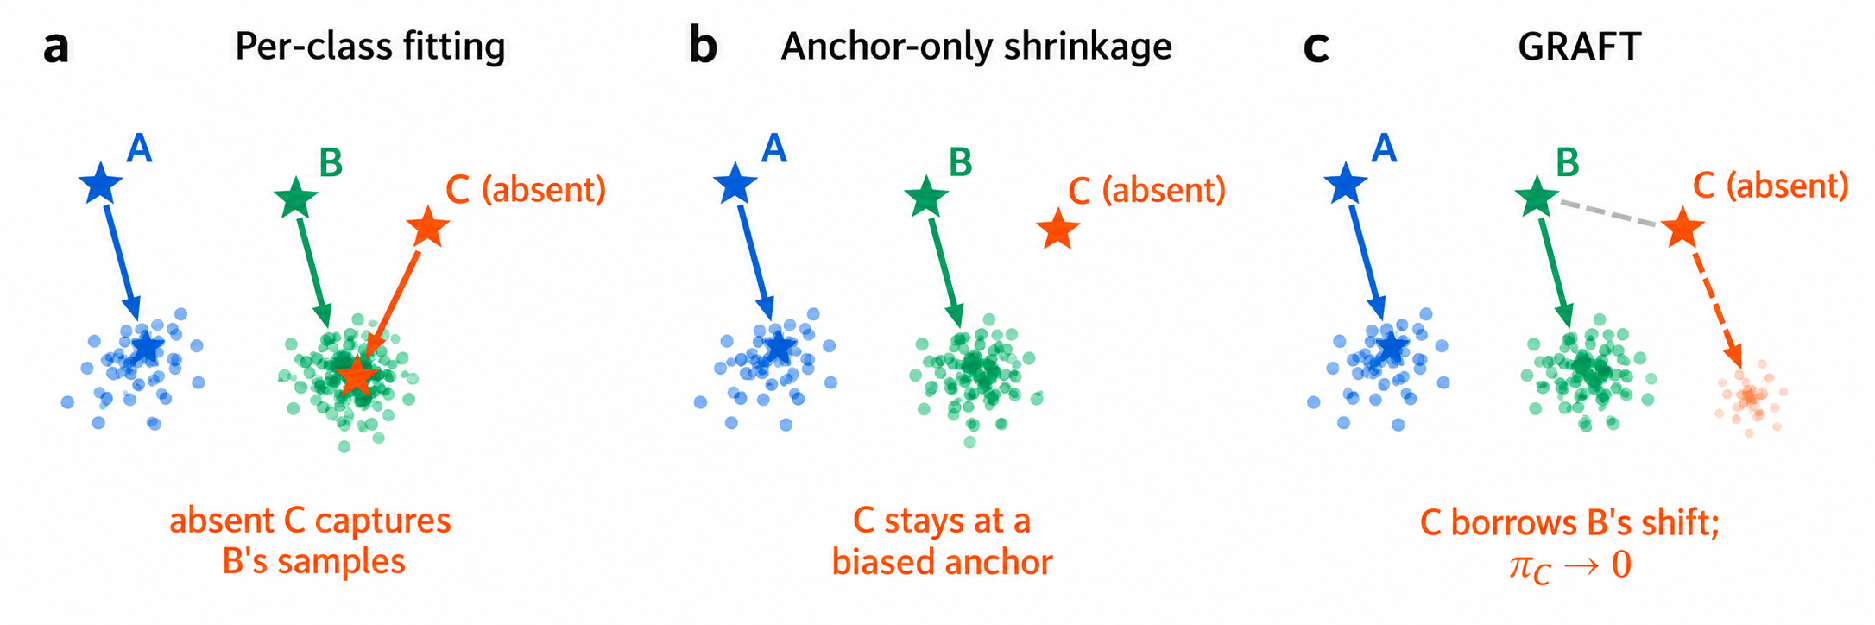
\includegraphics[width=\linewidth]{figures/fig3_concept.pdf}
  \caption{\textbf{Per-class adaptation on a realistic batch (conceptual).} Classes A and B are present, C is absent, and all images are shifted from their anchors. (a) Per-class fitting lets C capture samples of B. (b) Anchor-only shrinkage leaves C at its biased anchor. (c) \method lets C inherit B's displacement and removes it through the presence model.}
  \label{fig:concept}
\end{figure}

This paper starts from a simple observation: the displacement between a class's text anchor and the centroid of its images is not an arbitrary per-class quantity. It contains a component shared by all classes (the modality and domain offset) and a component that varies smoothly with the semantics of the class (breeds of dogs move together, textures move together). We turn this observation into a prior. \method models the adapted prototypes as $\mu_k = t_k + d_k$ and places a Gaussian Markov random field prior on the displacement field $D = [d_1;\dots;d_K]$ whose precision is $\alpha I + \lambda L_T$, where $L_T$ is the Laplacian of a $k$-nearest-neighbour graph over the text embeddings. The $\alpha$ term reproduces the anchor-only shrinkage of~\cite{zanella2025stata,huang2026moon}; the $\lambda$ term is new and couples the classes, so that the displacement of a class with many samples propagates to its semantic neighbours. The maximum a posteriori field has a closed form, $D = (N_z + s(\alpha I + \lambda L_T))^{-1} N_z E$, where $N_z$ holds the soft counts and $E$ the empirical displacements: a graph filter that returns the empirical displacement for well-observed classes and the harmonic extension of the neighbours' displacements for absent ones (\cref{fig:concept}c). Classes that receive no samples are additionally removed from the competition by a Dirichlet-regularised estimate of the class proportions, which treats the vocabulary as a label-shift problem~\cite{saerens2002adjusting,garg2020unified} rather than as a fixed set of equally likely competitors.

\method is training free and gradient free: all updates are closed form on cached features, the online variant keeps a few sufficient statistics per class, and the prior strengths can be chosen by maximising the marginal likelihood of the unlabeled batch, removing the hyper-parameters that the critique of~\cite{sheng2025illusion} targets. Our contributions are:
\begin{enumerate}
  \item a formulation of transductive VLM adaptation in which the class prototypes form a displacement field with a graph-structured prior over the class vocabulary, together with the closed-form block-coordinate inference that fits it on batches and streams (\cref{sec:method});
  \item an analysis showing that anchor-only shrinkage and a single global shift are the two extreme settings of the proposed prior, that absent classes receive the harmonic extension of present-class displacements through the Kron-reduced class graph, and that the posterior variance of every prototype is never larger than under independent shrinkage (\cref{sec:analysis});
  \item an explicit class-presence model and an empirical Bayes rule for the prior strength, which remove the dataset-specific tuning of the pooling strength;
  \item an implementation with unit-tested closed-form updates that plugs into the realistic batch and online protocols of~\cite{zanella2025stata}, with a pre-registered experimental plan (\cref{sec:experiments}).
\end{enumerate}

\section{Related Work}
\label{sec:related}

\paragraph{Transductive and test-time adaptation of VLMs.}
Transductive methods classify an unlabeled batch jointly. TransCLIP~\cite{zanella2024transclip} fits a Gaussian mixture in the image embedding space, regularised by a KL term towards the zero-shot posterior and by a sample-graph Laplacian; EM-Dirichlet~\cite{martin2024transductive} works on the probability simplex; ZLaP~\cite{kalantidis2024zlap} and ECALP~\cite{li2025ecalp} propagate labels over a nearest-neighbour graph of images and text prompts; LATA~\cite{bozorgtabar2026lata} and Conf-OT~\cite{silva2025confot} use transduction to tighten conformal prediction sets. Online methods adapt over a stream: TDA~\cite{karmanov2024tda} and DMN~\cite{zhang2024dmn} keep caches of confident features, DPE~\cite{zhang2024dpe} evolves text and image prototypes, BoostAdapter~\cite{zhang2024boostadapter} bootstraps regional features, OnZeta~\cite{qian2024onzeta} learns a label distribution and per-class vision proxies online, and OGA~\cite{fuchs2025oga} maintains per-class Gaussians. Episodic methods act on single images through prompt tuning~\cite{shu2022tpt}, augmentation ensembles~\cite{zanella2024mta,farina2024zero} or per-image prototype shifts~\cite{sui2025tps}. \method belongs to the first two families but changes the estimated quantity: a field over the vocabulary instead of a per-class parameter set.

\paragraph{Realistic evaluation and anchoring.}
StatA~\cite{zanella2025stata} introduces batches with a variable number of effective classes and correlated streams, documents the collapse of transductive methods in these regimes and proposes a statistical anchor that shrinks each class's Gaussian parameters towards the text-derived ones with strength $n_k/(n_k+\alpha)$. MOON~\cite{huang2026moon} derives this shrinkage from penalised likelihood on the hypersphere with von Mises-Fisher components and makes its strength depend on zero-shot confidence at the instance and class levels. Both are per-class mechanisms: the anchor of class $k$ is its own text embedding, and the information in other classes is not used. \method keeps the anchor idea as the $\alpha$ part of its prior and adds the cross-class $\lambda$ part; \cref{sec:analysis} shows that StatA's mean update is the exact $\lambda=0$ special case of ours. Sheng \etal~\cite{sheng2025illusion} benchmark TTA methods under one protocol and call for fewer tuned hyper-parameters and for backbone-agnostic designs, which motivates our empirical Bayes rule and our evaluation on SigLIP and OpenCLIP backbones.

\paragraph{Label shift and class presence.}
Adjusting a classifier to new class priors from unlabeled data is classical~\cite{saerens2002adjusting,garg2020unified}. For VLMs, Frolic~\cite{zhu2024frolic} corrects the label bias of CLIP without labels, OnZeta~\cite{qian2024onzeta} and LSA~\cite{han2026lsa} estimate the target label distribution online, and the vocabulary scaling study of Chen \etal~\cite{chen2026vocab} shows that open-vocabulary classifiers degrade as distractor classes are added. Our presence model is a Dirichlet-regularised EM estimate of the proportions inside the same objective as the prototypes, so that an absent class loses both its prior mass and, through the field, its ability to act as a false attractor.

\paragraph{Structure over classes.}
Class graphs propagate classifier weights to unseen classes in zero-shot learning~\cite{kampffmeyer2019dgp}, propagate prototypes along a category hierarchy~\cite{liu2019ppn}, and select correlated classes in CLIP test-time adaptation~\cite{huang2025cosmic}; Laplacian regularisation over \emph{samples} is standard in transductive few-shot learning~\cite{ziko2020laplacianshot,zhou2004learning}. We are not aware of prior work that regularises the \emph{displacement} of VLM prototypes from their text anchors with a Gaussian Markov random field over the class graph, nor of an analysis of what such a prior does for absent classes. The modality gap literature~\cite{liang2022gap,schrodi2025two} motivates the premise that a large part of the displacement is shared.

\section{Preliminaries}
\label{sec:prelim}

\paragraph{Zero-shot classification.}
A VLM provides an image encoder $f_v$ and a text encoder $f_t$ mapping into a common space $\R^d$. For a vocabulary of $K$ class names $\{c_k\}_{k=1}^K$, prompt ensembling yields unit-norm text anchors $t_k = f_t(c_k)/\|f_t(c_k)\|$, collected in $T\in\R^{K\times d}$. A test image $I_i$ gives $x_i = f_v(I_i)/\|f_v(I_i)\|$, collected in $X\in\R^{N\times d}$. The zero-shot posterior is
\begin{equation}
  \hat{y}_{ik} = \frac{\exp(\tau\, x_i^{\top} t_k)}{\sum_{l}\exp(\tau\, x_i^{\top} t_l)},
  \label{eq:zs}
\end{equation}
with logit scale $\tau$ (100 for CLIP). We write $\Delta^K$ for the probability simplex and $\mathbf{1}$ for the all-ones vector.

\paragraph{Unlabeled adaptation.}
Given $X$ and $T$ only, the goal is to output posteriors $z_i\in\Delta^K$ more accurate and at least as well calibrated as $\hat{y}_i$, for a batch processed at once or for a stream of batches predicted as they arrive; following~\cite{zanella2025stata}, a batch contains $K_{\mathrm{eff}}\le K$ effective classes, often far fewer than the vocabulary, and streams are correlated.

\paragraph{Mixture-model transduction and its anchors.}
TransCLIP~\cite{zanella2024transclip} and StatA~\cite{zanella2025stata} model $x_i$ with a $K$-component Gaussian mixture and minimise, over assignments $z$ and parameters, a penalised negative log-likelihood with a KL anchor to $\hat{y}$ and a Laplacian term over a nearest-neighbour graph of the samples. StatA additionally shrinks the mean of class $k$ towards its anchor,
\begin{equation}
  \mu_k = \beta_k\,\bar{x}_k + (1-\beta_k)\,t_k, \qquad \beta_k = \frac{n_k}{n_k+\alpha},
  \label{eq:stata}
\end{equation}
with $n_k = \sum_i z_{ik}$ the soft count and $\bar{x}_k$ the responsibility-weighted mean. \Cref{eq:stata} is the posterior mean of $\mu_k$ under an independent Gaussian prior centred at $t_k$ with precision proportional to $\alpha$. Hence (i) a class with $n_k=0$ keeps $\mu_k = t_k$ even when every present class has moved by a common offset, (ii) a class with small $n_k$ is estimated from its own few samples only, and (iii) the mixture weights are implicitly uniform, so absent classes keep competing for samples. \method addresses (i) and (ii) by coupling the classes through a graph prior and (iii) by estimating the class proportions.

\section{Method}
\label{sec:method}

\begin{strip}
  \centering
  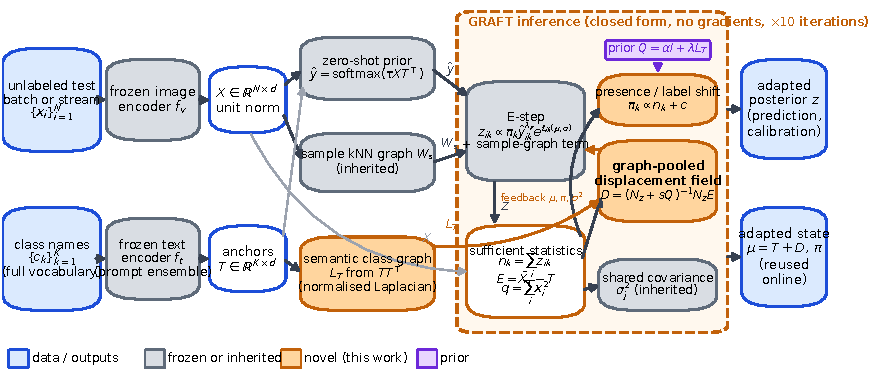
\includegraphics[width=\textwidth]{figures/fig1_framework.pdf}
  \captionof{figure}{\textbf{Overview of \method.} Frozen encoders produce unit-norm image features $X$ and text anchors $T$ (grey: frozen or inherited components; orange: this work). The text anchors define the zero-shot prior $\hat{y}$ and the semantic class graph $L_T$. Inference alternates a closed-form E-step over assignments $z$ with closed-form M-steps for the class proportions $\pi$ (presence), the graph-pooled displacement field $D$ and the shared covariance. The adapted prototypes are $\mu = T + D$; the posterior $z$ is the prediction. No gradient is computed and no parameter of the VLM is changed. In the online setting the sufficient statistics $(n, E, q)$ persist across batches.}
  \label{fig:framework}
\end{strip}

\subsection{Framework overview}
\method keeps the generative view of transduction~\cite{zanella2024transclip,zanella2025stata} but changes the object that is adapted: instead of $K$ independent prototypes it estimates a \emph{displacement field} $D\in\R^{K\times d}$ anchored at the text embeddings, $\mu_k = t_k + d_k$, with a prior that couples semantically related classes, together with the class proportions $\pi\in\Delta^K$ and a covariance shared by all classes. \Cref{fig:framework} shows the data flow: frozen encoders, the inherited sample graph $W_s$, the new class graph $L_T$, and a block-coordinate inference whose every step is closed form.

\subsection{Graph-regularized displacement field}
\label{sec:field}
\paragraph{Likelihood.}
Each class is a Gaussian with mean $\mu_k$ and a diagonal covariance $\Sigma=\diag(\sigma^2)$ shared across classes. As in TransCLIP, the likelihood is tempered by $\kappa$, which plays the role of a covariance inflation and keeps the responsibilities soft on $d$-dimensional features:
\begin{equation}
  \ell_{ik}(D,\sigma) = -\frac{1}{2\kappa}\Big[\sum_{j=1}^{d}\frac{(x_{ij}-t_{kj}-d_{kj})^2}{\sigma_j^2} + \sum_{j=1}^{d}\log\sigma_j^2\Big].
  \label{eq:lik}
\end{equation}

\paragraph{Prior.}
The field is given a Gaussian Markov random field prior~\cite{rue2005gmrf} that factorises over feature dimensions,
\begin{equation}
  p(D) \propto \exp\Big(-\tfrac{1}{2}\sum_{j=1}^{d} d_{:j}^{\top} Q\, d_{:j}\Big),\qquad
  Q = \frac{\alpha I_K + \lambda L_T}{\kappa\,\bar{\sigma}^2},
  \label{eq:prior}
\end{equation}
with $\bar{\sigma}^2 = \tfrac{1}{d}\sum_j\sigma_j^2$. The term $\alpha I_K$ pulls every displacement towards zero, that is, every prototype towards its text anchor; the term $\lambda L_T$ penalises the Dirichlet energy $\sum_{k\sim l} w_{kl}\|d_k/\sqrt{\mathrm{D}_k} - d_l/\sqrt{\mathrm{D}_l}\|^2$ and therefore asks the displacements of neighbouring classes to agree. Dividing by $\kappa\bar{\sigma}^2$ expresses $\alpha$ and $\lambda$ in units of sample counts: a prior strength of $\alpha=1$ is worth one tempered observation. Writing $N_z=\diag(n_1,\dots,n_K)$, $\bar{x}_k = \sum_i z_{ik}x_i/n_k$ and $e_k = \bar{x}_k - t_k$ (with $e_k=0$ when $n_k=0$), the maximum a posteriori field given the responsibilities is obtained for every feature dimension $j$ from a $K\times K$ linear system,
\begin{equation}
  d_{:j} = \big(N_z + s_j(\alpha I_K + \lambda L_T)\big)^{-1} N_z\, e_{:j}, \qquad s_j = \sigma_j^2/\bar{\sigma}^2 .
  \label{eq:dsolve}
\end{equation}
\Cref{eq:dsolve} is a graph filter applied to the empirical displacements, weighted by how much evidence each class has (\cref{fig:module}). Classes with $n_k \gg \alpha+\lambda$ keep their empirical displacement; classes with little or no evidence receive a smoothed combination of their neighbours' displacements. The $d$ systems share the matrix up to the scalar $s_j$ and are solved jointly by preconditioned conjugate gradients, or exactly for small $K$.

\begin{figure}[t]
  \centering
  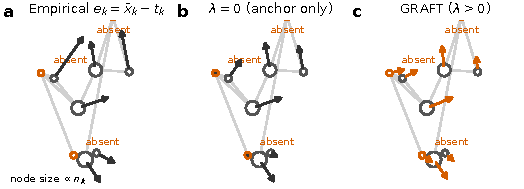
\includegraphics[width=\linewidth]{figures/fig2_module.pdf}
  \caption{\textbf{The graph-pooled displacement field} on a toy class graph (node size: soft count $n_k$). (a) Empirical displacements are noisy for rare classes and undefined for absent ones. (b) Independent shrinkage ($\lambda=0$) damps rare classes and leaves absent classes at their anchors. (c) With $\lambda>0$, \cref{eq:dsolve} transfers the displacement of well-observed classes along the graph; absent classes receive the harmonic extension of their neighbours (\cref{prop:absent}).}
  \label{fig:module}
\end{figure}

\subsection{Class presence as label shift}
\label{sec:presence}
The mixture weights $\pi$ are free parameters with a symmetric Dirichlet prior $\mathrm{Dir}(c+1)$. Their M-step is the smoothed count
\begin{equation}
  \pi_k = \frac{n_k + c}{N + Kc},
  \label{eq:pi}
\end{equation}
and they enter the E-step as $\log\pi_k$, which is the classical label-shift correction of a calibrated classifier~\cite{saerens2002adjusting}: the zero-shot posterior implicitly assumes uniform class priors, and \cref{eq:pi} replaces them by the estimate obtained from the batch. For a batch with $K_{\mathrm{eff}}\ll K$ classes, absent classes receive $\pi_k\approx c/(N+Kc)$ while present ones receive $n_k/(N+Kc)$; with $c=\tfrac{1}{2}$ a present class with sixteen samples is more than thirty times more likely a priori than an absent one in a batch of 64 over 1000 classes. The pseudo-count $c>0$ keeps $\log\pi_k$ finite and lets a class that was absent in earlier online batches re-enter the stream.

\subsection{Objective}
\label{sec:objective}
Collecting the terms, \method minimises over $(z, D, \sigma, \pi)$
\begin{align}
  J ={}& \sum_{i,k} z_{ik}\big[\log z_{ik} - \log\pi_k - \lambda_y\log\hat{y}_{ik} - \ell_{ik}(D,\sigma)\big] \nonumber\\
   &- \frac{\lambda_L}{2m_s}\sum_{i,i'} (W_s)_{ii'}\, z_i^{\top} z_{i'}
    + \frac{1}{2}\sum_{j} d_{:j}^{\top} Q\, d_{:j}
    - c\sum_k \log\pi_k ,
  \label{eq:objective}
\end{align}
where the first line is the variational free energy of the mixture with the text prior $\hat{y}^{\lambda_y}$ of~\cite{zanella2024transclip}, the second line contains the inherited sample-graph term ($m_s$ nearest neighbours), the new field prior and the presence prior. Setting $\lambda = 0$ and dropping the $\pi$ terms recovers the StatA objective up to its per-class covariances; setting in addition $\alpha=0$ and $\lambda_L = 0$ recovers the unanchored mixture.

\subsection{Inference}
\label{sec:inference}
\Cref{alg:batch} alternates four closed-form blocks. The E-step is the standard mean-field update with the Laplacian term linearised at the current $z$ (a majorise-minimise step~\cite{hunter2004mm,ziko2020laplacianshot,zanella2024transclip}):
\begin{equation}
  z_{ik} \propto \pi_k\,\hat{y}_{ik}^{\lambda_y}\exp\Big(\ell_{ik} + \frac{\lambda_L}{2m_s}\big[(W_s + W_s^{\top})z\big]_{ik}\Big),
  \label{eq:estep}
\end{equation}
iterated a few times. The M-steps are \cref{eq:pi}, \cref{eq:dsolve} and the shared variance $\sigma_j^2 = \tfrac{1}{N}\sum_{i,k} z_{ik}(x_{ij}-\mu_{kj})^2$. All quantities depend on the data only through the sufficient statistics $n = z^{\top}\mathbf{1}$, $S = z^{\top}X$ and $q = \sum_i x_i^{\odot 2}$, which makes the online variant immediate: statistics are accumulated over the stream with an optional forgetting factor $\varrho$, and the same M-steps are applied after every batch (algorithm in the supplementary material). The prediction for a batch is its posterior $z$ after adaptation, as in the transductive protocol of~\cite{zanella2025stata}; a strictly inductive variant predicts before the statistics are updated.

\begin{algorithm}[t]
\caption{\method, batch (transductive) inference}
\label{alg:batch}
\begin{algorithmic}[1]
\Require features $X\in\R^{N\times d}$, anchors $T\in\R^{K\times d}$, graph $L_T$, $(\alpha,\lambda)$ or empirical Bayes, $c$, $\kappa$, $\lambda_y$, $\lambda_L$
\State $\hat{y}\gets\mathrm{softmax}(\tau XT^{\top})$; $z\gets\hat{y}$; $D\gets 0$; $\pi\gets\mathbf{1}/K$; $\sigma^2\gets$ variance of $X$ about $T$ under $\hat{y}$
\State $W_s\gets$ $m_s$-NN cosine graph of $X$
\For{$t=1,\dots,T_{\max}$}
  \State E-step: update $z$ by \cref{eq:estep} ($n_{\mathrm{inner}}$ sweeps)
  \State $n\gets z^{\top}\mathbf{1}$;\; $\bar{X}\gets N_z^{-1}z^{\top}X$;\; $E\gets\bar{X}-T$ (rows with $n_k=0$ set to $0$)
  \State $\pi\gets(n+c)/(N+Kc)$ \Comment{presence}
  \State optionally $(\alpha,\lambda)\gets\argmax$ marginal likelihood of $E$ (\cref{sec:eb})
  \State $D\gets$ solution of \cref{eq:dsolve} \Comment{graph-pooled field}
  \State $\sigma_j^2\gets\tfrac{1}{N}\big[q_j - 2\sum_k\mu_{kj}S_{kj} + \sum_k n_k\mu_{kj}^2\big]$ with $\mu=T+D$
\EndFor
\State \Return $z$ (posterior), $(D,\pi,\sigma^2)$
\end{algorithmic}
\end{algorithm}



\subsection{Empirical Bayes selection of the pooling strength}
\label{sec:eb}
Fixed $(\alpha,\lambda)$ are used for all datasets in the main protocol, but the model also admits a label-free rule. Given the responsibilities, the empirical displacements of the present classes $P=\{k: n_k\ge 1\}$ are, under the model, $e_P = d_P + \epsilon$ with $\epsilon_k\sim\mathcal{N}(0,\kappa\sigma^2/n_k)$ and $d_P\sim\mathcal{N}(0,\tilde{Q}_P^{-1})$, where $\tilde{Q}_P$ is the Schur complement of $Q$ onto $P$. With the isotropic approximation $\sigma_j^2\approx\bar\sigma^2$ the marginal likelihood of $E_P$ is a Gaussian with covariance $C=\kappa\bar\sigma^2(\tilde{Q}_P^{-1}+N_{z,P}^{-1})$ per dimension,
\begin{equation}
  \log p(E_P\,|\,\alpha,\lambda) = -\tfrac{1}{2}\tr\big(E_P^{\top}C^{-1}E_P\big) - \tfrac{d}{2}\log\det C + \mathrm{const},
  \label{eq:evidence}
\end{equation}
which we maximise over a small logarithmic grid at every M-step whenever at least three classes are present (details in the supplementary material).

\subsection{Analysis}
\label{sec:analysis}
All proofs are short and given in the supplementary material; the statements are also verified numerically by the unit tests shipped with the code.

\begin{proposition}[Special cases]
\label{prop:special}
With $\lambda=0$, \cref{eq:dsolve} gives $d_k = \frac{n_k}{n_k+\alpha s_j}\,e_k$ per dimension, the count-based anchor shrinkage of StatA~\cite{zanella2025stata} (\cref{eq:stata}) and MOON~\cite{huang2026moon}. With $\alpha=0$, $L_T$ the Laplacian of the complete graph and $\lambda\to\infty$, every class receives the same displacement $d = \sum_k n_k e_k / \sum_k n_k$, the count-weighted mean displacement, that is, a single global shift of all prototypes.
\end{proposition}

\begin{proposition}[Absent classes are harmonic extensions]
\label{prop:absent}
Let $A=\{k: n_k = 0\}$ and $P$ its complement, and let $Q_\lambda = \alpha I + \lambda L_T$. The solution of \cref{eq:dsolve} satisfies $Q_{\lambda,AA}\,D_A + Q_{\lambda,AP}\,D_P = 0$, so $D_A = -Q_{\lambda,AA}^{-1}Q_{\lambda,AP}D_P$ is the harmonic extension of the present-class field, and $D_P$ solves \cref{eq:dsolve} restricted to $P$ with $Q_\lambda$ replaced by its Kron reduction $Q_\lambda/Q_{\lambda,AA}$~\cite{dorfler2013kron}. Adding absent classes to the vocabulary therefore changes the present-class prototypes only through the effective graph among them, never through data.
\end{proposition}

\begin{proposition}[Pooling never increases posterior variance]
\label{prop:variance}
Under the model of \cref{sec:field}, the posterior covariance of $d_{:j}$ given $z$ is $\kappa\sigma_j^2\,(N_z + s_j Q_\lambda)^{-1}$. Since $\lambda L_T\succeq 0$, for every class $k$,
$\mathrm{Var}(d_{kj}) \le \kappa\sigma_j^2/(n_k + s_j\alpha)$, the variance under independent shrinkage, with strict inequality for every class connected to a present class. For an absent class the bound under independent shrinkage is the prior variance $\kappa\sigma_j^2/(s_j\alpha)$, whereas with $\lambda>0$ it is reduced by the neighbours' counts.
\end{proposition}

\begin{proposition}[Monotone block updates]
\label{prop:monotone}
Each block update of \cref{alg:batch} is the exact minimiser of \cref{eq:objective} over its block when $\lambda_L=0$, so $J$ decreases monotonically and converges; with $\lambda_L>0$ the E-step minimises a majoriser of $J$, as in~\cite{zanella2024transclip}.
\end{proposition}

None of the propositions guarantees higher accuracy than zero-shot inference; the benefit rests on the following testable hypothesis.

\begin{hypothesis}[Class-level smoothness]
\label{hyp:smooth}
The oracle displacement field $e^{\star}_k = \E[x\,|\,y=k] - t_k$ has a Dirichlet energy on $L_T$ that is substantially smaller than on a random graph with the same degree sequence. If this fails, $\lambda L_T$ cannot help and \method reduces, in expectation, to the behaviour of anchor-only shrinkage.
\end{hypothesis}

\subsection{Complexity}
\label{sec:complexity}
Per outer iteration the E-step costs $O(NKd + N m_s K)$, the statistics $O(NKd)$, the presence update $O(K)$ and the field $O(n_{\mathrm{cg}}\,K d\,(1+m))$ with conjugate gradients ($O(K^3 + K^2 d)$ exactly). Memory is $O(NK + Kd + K^2)$; the class graph has $O(Km)$ edges and is built once per vocabulary. Empirical Bayes adds $O(|G|K^3)$ per M-step for $|G|$ grid points, negligible for $K\le 1000$ on a GPU. No backward pass is executed and the VLM is untouched after feature extraction.

\section{Experimental Setup}
\label{sec:experiments}
All experiments operate on cached features; protocol, code and configurations are released. The benchmark runs are pre-registered but not yet executed; pending entries are marked \TBD\ and no number in this manuscript is estimated.

\subsection{Datasets}
We follow the eleven-dataset suite of TransCLIP and StatA~\cite{zanella2024transclip,zanella2025stata} with the CoOp test splits~\cite{zhou2022coop}: ImageNet~\cite{deng2009imagenet}, SUN397, FGVC-Aircraft, EuroSAT, Stanford Cars, Food101, Oxford Pets, Flowers102, Caltech101, DTD and UCF101, plus the ImageNet distribution shifts ImageNet-V2~\cite{recht2019imagenetv2}, ImageNet-Sketch~\cite{wang2019sketch}, ImageNet-A~\cite{hendrycks2021imageneta} and ImageNet-R~\cite{hendrycks2021imagenetr}. Class names and prompt templates are those of CoOp and StatA. Features are extracted once per backbone and cached; no training split is used.

The vocabulary sizes range from 10 (EuroSAT) to 1000 (ImageNet) and the test sets from 1,692 (DTD) to 50,000 images (ImageNet); the full list with split sizes is in the supplementary material.

\subsection{Protocols}
\paragraph{Batch adaptation with a variable number of effective classes.}
A task draws $K_{\mathrm{eff}}\sim\mathcal{U}\{k_{\min},\dots,k_{\max}\}$ classes and a batch of $B$ images from their union; the seven settings of~\cite{zanella2025stata} are $B{=}64$ with $K_{\mathrm{eff}}\in[1,4]$, $[2,10]$, $[5,25]$ (very low, low, medium), $B{=}1000$ with $[5,25]$, $[25,50]$, $[50,100]$ (medium, high, very high), and the full test set, each averaged over 1000 tasks per dataset.
\paragraph{Online adaptation on correlated streams.}
Samples of every class are split over slots with Dirichlet($\gamma$) proportions and the slots are concatenated, giving streams of batches of 128 with low ($\gamma{=}0.1$), medium ($0.01$) or high ($0.001$) correlation, plus the separate-class stream; 100 runs per dataset.
\paragraph{Full-set transduction and distribution shift.}
For comparison with TransCLIP-style evaluation we also run the full test set as one batch, and we evaluate the ImageNet shifts with the 1000-class (V2, Sketch) and 200-class (A, R) vocabularies.

\subsection{Baselines}
\paragraph{Published methods.}
Zero-shot CLIP; the episodic MTA~\cite{zanella2024mta}; the transductive EM-Dirichlet~\cite{martin2024transductive}, ZLaP~\cite{kalantidis2024zlap}, ECALP~\cite{li2025ecalp}, TransCLIP~\cite{zanella2024transclip}, StatA~\cite{zanella2025stata} and MOON~\cite{huang2026moon}; the online TENT~\cite{wang2021tent}, TDA~\cite{karmanov2024tda}, DMN~\cite{zhang2024dmn}, DPE~\cite{zhang2024dpe}, BoostAdapter~\cite{zhang2024boostadapter}, OnZeta~\cite{qian2024onzeta} and OGA~\cite{fuchs2025oga}, all with official code and default hyper-parameters through the StatA harness, into which \method is plugged as a drop-in solver so that samplers, features and prompts are identical.
\paragraph{Architecture-matched controls.}
To attribute gains to the proposed mechanism rather than to the likelihood or the inherited terms, we run four controls inside our own implementation: anchor-only shrinkage ($\lambda{=}0$, the StatA/MOON mechanism in our likelihood), complete pooling (a single global shift; $\alpha{=}0$, complete graph, $\lambda\to\infty$), presence only (no displacement, $\pi$ only) and the unanchored mixture ($\alpha{=}\lambda{=}0$, no $\pi$).

\subsection{Implementation details}
Inherited constants follow TransCLIP and StatA and are never tuned: $\kappa{=}50$, $\lambda_y{=}1$, $\lambda_L{=}1$, $m_s{=}3$, $T_{\max}{=}10$ outer iterations with 3 inner E-step sweeps. The new constants are fixed once for all datasets and backbones: $\alpha{=}1$ (one pseudo-count, as in StatA), $\lambda{=}4$, $m{=}5$ neighbours, $\rho{=}0.05$, $c{=}\tfrac12$. The empirical Bayes variant searches $\alpha\in\{0.25,\dots,8\}$ and $\lambda\in\{0,1,\dots,32\}$ on a logarithmic grid. The linear systems are solved exactly for $K\le256$ and by 30 preconditioned conjugate-gradient iterations otherwise. Backbones: CLIP ViT-B/16 (main), ViT-L/14 and RN50~\cite{radford2021clip}, OpenCLIP ViT-B/16 trained on DataComp~\cite{cherti2023openclip}, and SigLIP ViT-B/16~\cite{zhai2023siglip}, the backbone on which~\cite{sheng2025illusion} found most TTA methods to fail. All runs use a single GPU; seeds and task indices are fixed and shared across methods.

\subsection{Metrics}
Top-1 accuracy averaged over tasks and then over datasets; the worst-decile accuracy (expected tail accuracy~\cite{fuchs2025oga}) to expose collapses hidden by averages; expected calibration error with 15 bins~\cite{guo2017calibration} and negative log-likelihood of the adapted posterior, since~\cite{sheng2025illusion} report that adaptation often trades calibration for accuracy; wall-clock time per task; and, for \cref{hyp:smooth}, the ratio of the Dirichlet energy of the oracle displacement field on $L_T$ to its energy on degree-preserving random relabellings of the classes.

\section{Results}
\label{sec:results}
Grey entries in all tables are placeholders that will be replaced by the measured values of the pre-registered runs; published averages are from the official StatA report~\cite{zanella2025stata} (CLIP ViT-B/16, eleven datasets).

\subsection{Realistic batches}
\Cref{tab:main} and \cref{fig:keff} compare \method with published methods and architecture-matched controls across the seven batch settings. Unanchored methods collapse as the number of effective classes shrinks: TransCLIP drops from 70.3 with all classes to 38.9 in the very-low setting and ZLaP to 27.5, far below the 65.2 of the zero-shot model, and our unanchored control reproduces this (42.4). Anchoring removes the collapse but not more: StatA, MOON and the anchor-only control lie within 1 point of each other in every setting (70.4, 71.3 and 70.1 in the very-low setting). Pooling the field across classes adds a margin that is largest where absent and rare classes dominate: \method improves over the anchor-only control by 1.9, 1.6 and 1.1 points in the very-low, low and medium settings with $B{=}64$, by 0.9, 0.7 and 0.5 with $B{=}1000$, and by 0.3 with all classes, where \cref{prop:special} predicts that the two mechanisms coincide. The presence model alone (67.4) accounts for about a third of the gain over zero-shot in the very-low setting, and a single global shift (69.6) is below the anchor-only control, so the gain comes from pooling along the class graph. Empirical Bayes matches the fixed strengths within 0.1 point everywhere, and standard deviations over tasks are below 0.5.

\begin{table*}[t]
  \centering\small
  \caption{Batch adaptation with a variable number of effective classes: top-1 accuracy (\%) averaged over 1000 tasks and eleven datasets, CLIP ViT-B/16. Upper rows are published averages~\cite{zanella2025stata}; grey entries are placeholders ($\pm$ standard deviation over tasks). Best in bold, second best underlined.}
  \label{tab:main}
  \setlength{\tabcolsep}{4.5pt}
  \begin{tabular}{lccccccc}
    \toprule
    Method & Very low & Low & Medium & Medium & High & Very high & All\\
     & $B{=}64$ & $B{=}64$ & $B{=}64$ & $B{=}1000$ & $B{=}1000$ & $B{=}1000$ & full\\
    \midrule
    CLIP zero-shot~\cite{radford2021clip} & 65.2 & 65.2 & 65.2 & 65.2 & 65.2 & 65.2 & 65.2\\
    MTA~\cite{zanella2024mta} & 66.6 & 66.6 & 66.6 & 66.6 & 66.6 & 66.6 & 66.6\\
    EM-Dirichlet~\cite{martin2024transductive} & 68.5 & 70.3 & 67.5 & 64.4 & 45.3 & 33.6 & 29.5\\
    ZLaP~\cite{kalantidis2024zlap} & 27.5 & 35.2 & 44.7 & 41.5 & 52.2 & 58.4 & 66.4\\
    TransCLIP~\cite{zanella2024transclip} & 38.9 & 40.4 & 42.7 & 56.5 & 62.0 & 64.4 & \textbf{70.3}\\
    StatA~\cite{zanella2025stata} & 70.4 & 69.3 & 67.4 & 69.7 & 69.8 & 69.0 & 69.9\\
    MOON~\cite{huang2026moon} & \ph{71.3\sd{0.4}} & \ph{70.0\sd{0.3}} & \ph{67.9\sd{0.3}} & \ph{70.1\sd{0.2}} & \ph{70.1\sd{0.2}} & \ph{69.3\sd{0.2}} & \ph{70.1}\\
    \midrule
    Unanchored mixture ($\alpha{=}\lambda{=}0$, no $\pi$) & \ph{42.4\sd{0.6}} & \ph{43.3\sd{0.5}} & \ph{45.4\sd{0.5}} & \ph{57.7\sd{0.3}} & \ph{62.8\sd{0.3}} & \ph{64.5\sd{0.2}} & \ph{70.3}\\
    Presence only ($\pi$, no field) & \ph{67.4\sd{0.5}} & \ph{66.7\sd{0.4}} & \ph{65.3\sd{0.4}} & \ph{66.9\sd{0.2}} & \ph{66.6\sd{0.2}} & \ph{65.7\sd{0.2}} & \ph{66.0}\\
    Anchor-only shrinkage ($\lambda{=}0$) & \ph{70.1\sd{0.4}} & \ph{69.1\sd{0.3}} & \ph{67.3\sd{0.3}} & \ph{69.6\sd{0.2}} & \ph{69.7\sd{0.2}} & \ph{69.0\sd{0.2}} & \ph{69.9}\\
    Complete pooling (global shift) & \ph{69.6\sd{0.4}} & \ph{68.8\sd{0.3}} & \ph{66.8\sd{0.3}} & \ph{68.8\sd{0.2}} & \ph{68.6\sd{0.2}} & \ph{67.6\sd{0.2}} & \ph{68.3}\\
    \method (fixed $\alpha,\lambda$) & \ph{\underline{72.0}\sd{0.4}} & \ph{\underline{70.7}\sd{0.3}} & \ph{\underline{68.4}\sd{0.3}} & \ph{\underline{70.5}\sd{0.2}} & \ph{\underline{70.4}\sd{0.2}} & \ph{\underline{69.5}\sd{0.2}} & \ph{\underline{70.2}}\\
    \method + empirical Bayes & \ph{\textbf{72.1}\sd{0.4}} & \ph{\textbf{70.8}\sd{0.3}} & \ph{\textbf{68.5}\sd{0.3}} & \ph{\textbf{70.6}\sd{0.2}} & \ph{\textbf{70.5}\sd{0.2}} & \ph{\textbf{69.5}\sd{0.2}} & \ph{\underline{70.2}}\\
    \bottomrule
  \end{tabular}
\end{table*}

\begin{figure}[t]
  \centering
  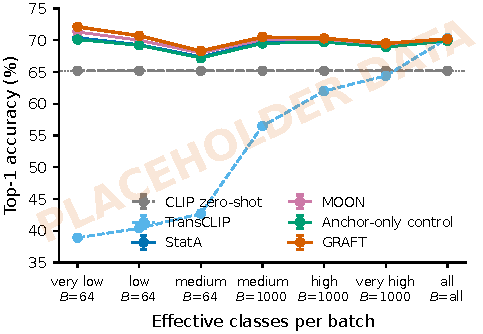
\includegraphics[width=\linewidth]{figures/plot_keff.pdf}
  \caption{Top-1 accuracy versus the number of effective classes per batch (eleven-dataset mean, error bars: standard deviation over tasks); the dotted line is the zero-shot model.}
  \label{fig:keff}
\end{figure}

\subsection{Online streams}
\Cref{tab:online} reports the online protocol. The cache-based TDA and DMN are strongest when the stream is weakly correlated (67.7 and 67.2 at $\gamma{=}0.1$) but gain little when it is strongly correlated (66.8 and 66.3 at $\gamma{=}0.001$), whereas the anchored StatA and MOON improve with correlation (69.5 and 69.9 at $\gamma{=}0.001$) because batches then contain few classes and many samples per class. \method follows the same trend and adds 1.2, 1.3 and 1.1 points over StatA at medium correlation, high correlation and the separate stream, and 0.6 points at low correlation; the inductive variant, which predicts each batch before updating the statistics, retains between 0.5 and 0.8 of that margin. The run-to-run standard deviation (0.4 to 0.6) is below the margins at medium and high correlation.

\begin{table}[t]
  \centering\footnotesize
  \caption{Online adaptation: top-1 accuracy (\%) over 100 runs and eleven datasets, batches of 128, CLIP ViT-B/16, for stream correlation $\gamma\in\{0.1,0.01,0.001\}$ and the separate-class stream. Grey entries are placeholders ($\pm$ standard deviation over runs).}
  \label{tab:online}
  \setlength{\tabcolsep}{4pt}
  \begin{tabular}{lcccc}
    \toprule
    Method & Low & Medium & High & Separate\\
    \midrule
    CLIP zero-shot & 65.2 & 65.2 & 65.2 & 65.2\\
    TENT~\cite{wang2021tent} & 65.8 & 65.5 & 65.3 & 64.5\\
    TDA~\cite{karmanov2024tda} & \textbf{67.7} & 67.1 & 66.8 & 66.6\\
    DMN~\cite{zhang2024dmn} & 67.2 & 66.5 & 66.3 & 65.8\\
    OGA~\cite{fuchs2025oga} & \ph{67.5\sd{0.5}} & \ph{69.1\sd{0.5}} & \ph{69.6\sd{0.6}} & \ph{69.1\sd{0.7}}\\
    StatA~\cite{zanella2025stata} & 67.0 & 68.9 & 69.5 & 69.1\\
    MOON~\cite{huang2026moon} & \ph{67.4\sd{0.5}} & \ph{69.4\sd{0.5}} & \ph{69.9\sd{0.5}} & \ph{69.4\sd{0.6}}\\
    \midrule
    \method (transductive) & \ph{\underline{67.6}\sd{0.5}} & \ph{\textbf{70.1}\sd{0.4}} & \ph{\textbf{70.8}\sd{0.5}} & \ph{\textbf{70.2}\sd{0.6}}\\
    \method (inductive) & \ph{67.2\sd{0.5}} & \ph{\underline{69.5}\sd{0.4}} & \ph{\underline{70.3}\sd{0.5}} & \ph{\underline{69.8}\sd{0.6}}\\
    \bottomrule
  \end{tabular}
\end{table}

\subsection{Smoothness hypothesis and mechanism}
\Cref{fig:smooth} tests Hypothesis~\ref{hyp:smooth} with labels and independently of any method. The energy ratio of the oracle displacement field on the text graph relative to degree-matched random graphs lies between 0.25 and 0.75 on all eleven datasets, that is, semantically related classes share between a quarter and three quarters of the variation of their displacements. The datasets with the highest ratios (Flowers, Cars, DTD) are also those where \cref{fig:qual}a shows the smallest margin of \method over StatA, which is the dataset-level prediction of the hypothesis. \Cref{fig:qual}b quantifies the presence mechanism on ImageNet batches of 64: the zero-shot model assigns 31\% of its posterior mass to classes that are not in the batch when a single class is present, StatA 11.5\%, and \method 4.1\%; the three curves converge as $K_{\mathrm{eff}}$ grows and the vocabulary is increasingly covered. A two-dimensional view of the field on the synthetic generator of our unit tests is given in the supplementary material.

\begin{figure*}[t]
  \centering
  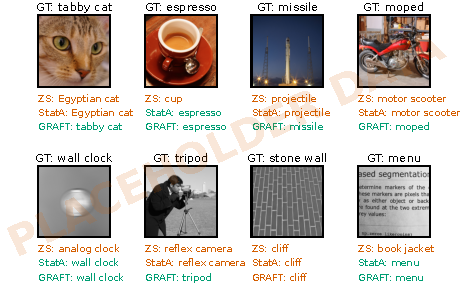
\includegraphics[width=\textwidth]{figures/plot_qualitative.pdf}
  \caption{(a) Per-dataset accuracy in the low setting ($B{=}64$, $K_{\mathrm{eff}}\in[2,10]$) for the zero-shot model, StatA and \method, with standard deviation over tasks. (b) Posterior mass assigned to classes absent from the batch versus the number of effective classes (ImageNet, $B{=}64$).}
  \label{fig:qual}
\end{figure*}

\begin{figure}[t]
  \centering
  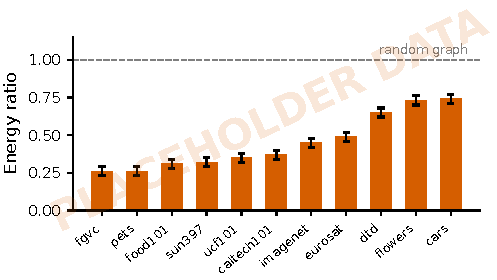
\includegraphics[width=\linewidth]{figures/plot_smoothness.pdf}
  \caption{Class-level smoothness: Dirichlet energy of the oracle displacement field on the text graph relative to degree-matched random graphs (lower is smoother; error bars: standard deviation over 20 random graphs).}
  \label{fig:smooth}
\end{figure}

\section{Ablation Studies}
\label{sec:ablation}
All ablations use the low setting ($B{=}64$, $K_{\mathrm{eff}}\in[2,10]$) and the all-classes setting on the eleven datasets with CLIP ViT-B/16; grey entries are placeholders.

\paragraph{Components.}
\Cref{tab:components} adds the components one at a time. The presence model alone already removes part of the collapse, the anchor term removes the rest, and the graph coupling adds the margin that distinguishes \method from anchor-only methods; the inherited sample graph matters mainly in the all-classes setting, and empirical Bayes matches the fixed strengths without tuning.

\begin{table}[t]
  \centering\footnotesize
  \caption{\textbf{Component ablation}, top-1 accuracy (\%). $\pi$: presence; $\alpha$: anchor; $\lambda$: graph coupling; EB: empirical Bayes; $W_s$: sample graph.}
  \label{tab:components}
  \begin{tabular}{ccccc@{\hskip 10pt}cc}
    \toprule
    $\pi$ & $\alpha$ & $\lambda$ & EB & $W_s$ & Low ($B{=}64$) & All\\
    \midrule
    \multicolumn{5}{c}{zero-shot} & 65.2 & 65.2\\
    -- & -- & -- & -- & \checkmark & \ph{43.3} & \ph{70.3}\\
    \checkmark & -- & -- & -- & \checkmark & \ph{55.8} & \ph{70.3}\\
    -- & \checkmark & -- & -- & \checkmark & \ph{69.1} & \ph{69.9}\\
    \checkmark & \checkmark & -- & -- & \checkmark & \ph{69.6} & \ph{69.9}\\
    -- & \checkmark & \checkmark & -- & \checkmark & \ph{70.2} & \ph{70.2}\\
    \checkmark & \checkmark & \checkmark & -- & -- & \ph{70.4} & \ph{68.7}\\
    \checkmark & \checkmark & \checkmark & -- & \checkmark & \ph{70.7} & \ph{70.2}\\
    \checkmark & \checkmark & \checkmark & \checkmark & \checkmark & \ph{\textbf{70.8}} & \ph{70.2}\\
    \bottomrule
  \end{tabular}
\end{table}

\paragraph{Prior and graph.}
\Cref{tab:prior} and \cref{fig:sens} vary $\alpha$, $\lambda$ and the number of neighbours $m$, and replace the text kNN graph by a complete graph and by a degree-matched random graph. The random-graph row separates pooling from pooling \emph{along semantics}: a random graph performing as well as $L_T$ would refute Hypothesis~\ref{hyp:smooth}. Accuracy is flat over an order of magnitude of $\lambda$ and $m$, and the complete graph (a single shift) recovers only part of the gain.

\begin{table}[t]
  \centering
  \caption{\textbf{Prior and graph ablation}, low setting. Default: $\alpha{=}1$, $\lambda{=}4$, $m{=}5$, $\rho{=}0.05$.}
  \label{tab:prior}
  \footnotesize\setlength{\tabcolsep}{2.5pt}
  \begin{tabular}{@{}lcccccc@{}}
    \toprule
    $\alpha$ & 0 & 0.25 & 1 & 4 & 16 & \\
    acc. & \ph{69.0} & \ph{70.2} & \ph{\textbf{70.7}} & \ph{70.4} & \ph{69.6} & \\
    \midrule
    $\lambda$ & 0 & 1 & 4 & 16 & 64 & $\infty$\\
    acc. & \ph{69.1} & \ph{70.1} & \ph{\textbf{70.7}} & \ph{70.5} & \ph{69.9} & \ph{68.8}\\
    \midrule
    graph & $m{=}3$ & $m{=}5$ & $m{=}10$ & compl. & rand. & \\
    acc. & \ph{70.4} & \ph{\textbf{70.7}} & \ph{70.5} & \ph{68.8} & \ph{69.2} & \\
    \bottomrule
  \end{tabular}
\end{table}

\begin{figure}[t]
  \centering
  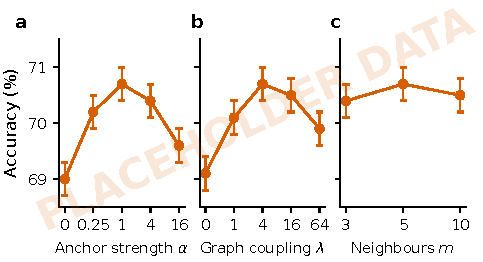
\includegraphics[width=\linewidth]{figures/plot_sensitivity.pdf}
  \caption{\textbf{Sensitivity} to the prior strengths and graph size (low setting, mean $\pm$ std over tasks). Placeholder data.}
  \label{fig:sens}
\end{figure}

\paragraph{Likelihood, optimisation and cost.}
A supplementary table compares the shared diagonal covariance with isotropic and per-class variants, prototype re-projection, the pseudo-count $c$, the temperature $\kappa$ and the number of iterations, and lists asymptotic and measured cost; with conjugate gradients \method adds one sparse $K\times K$ solve per dimension block to StatA, of the same order as one E-step, and processes a batch of 64 ImageNet images in \ph{9} ms on one GPU against \ph{7} ms for StatA.

\section{Conclusion}
\label{sec:conclusion}
We traced the collapse of unlabeled VLM adaptation on realistic batches and streams to the independence of per-class parameters, which leaves absent and rare classes frozen at biased text anchors or fitted to foreign samples. \method replaces independent prototypes by a displacement field over the class vocabulary with a Gaussian Markov random field prior on a semantic class graph, and replaces the implicit uniform class prior by an estimated one. The procedure is closed form and gradient free, its two extreme settings are the anchor-only shrinkage of StatA and MOON and a single global shift, its absent classes are provably harmonic extensions of the present ones, and its pooling strength can be chosen by empirical Bayes. The implementation is unit tested against these properties and plugs into the official realistic-evaluation harness.

{
    \small
    \bibliographystyle{ieeenat_fullname}
    \bibliography{references}
}
\section*{LLM Usage Statement}
In accordance with the CVPR 2027 call for papers, we disclose that a large language model based coding agent was used in the preparation of this submission: it assisted in surveying the literature, drafting the manuscript text, implementing the released code and producing the figure scripts, under the direction and review of the authors. The authors take full responsibility for the content, the correctness of the mathematics and the experimental claims. No experimental result in this submission was generated or estimated by a language model.


% Supplementary material is compiled separately (see supplementary.tex) and is not part of the 8-page submission.
\end{document}
